\section{Derivation of a MOSFET Small Signal Model}
\begin{frame}{Derivation: Notational Conventions}
    \begin{itemize}
        \item DC quantities are labeled with UPPERCASE variables and UPPERCASE subindices: 
        $V_{\mathrm{GS}}$
        \item Pure AC quantities are labeled with lowercase variables and lowercase subindices: 
        $v_{\mathrm{gs}}$
        \item Superpositions of both quantities are labeled with lowercase variables and 
        UPPERCASE subindices: $v_{\mathrm{GS}}=V_{\mathrm{GS}}+v_{\mathrm{gs}}$
    \end{itemize}
    \begin{figure}
        \centering
        \includegraphics{../plots/notational_convention.pdf}
        \caption{Notational conventions for DC and AC quantities.}
        \label{fig:signal_convention}
    \end{figure}
\end{frame}
\note[itemize]{
    \item Entering small signal theory
    \item Superimposed quantity
    \item DC: direct current
    \item AC: alternating current
}
    

\begin{frame}{Derivation: MOSFET Current-Voltage Characteristics}
    \vspace{0.5cm}
    \begin{figure}
        \centering
        \includegraphics{../plots/cv_characteristics.pdf}
        \caption{MOSFET current-voltage characteristics. Left: saturation drain current 
        as a function of gate voltage. Right: drain current as a function of 
        drain voltage for different gate voltages.}
        \label{fig:mosfet_characteristics}
    \end{figure}
    \begin{itemize}
        \item Require saturation-region operation: $V_{\mathrm{DS}}\gg V_{\mathrm{GS}}-V_{\mathrm{t}}$
        \item In this regime, the following current-voltage characteristics are valid:
        $i_{\mathrm{drain}}=\frac{1}{2}k_{\mathrm{n}}(v_{\mathrm{gate}}-V_{\mathrm{t}})^{2}$, 
        $i_{\mathrm{gate}}=0$
    \end{itemize}
\end{frame}
\note[itemize]{
    \item Drain- and gate- voltage are relative to source.
    \item Depending on mode of operation, different behavior, different models
    \item Parabola intersects curve for $v_\mathrm{drain}=v_\mathrm{gate}-V_\mathrm{t}$
    \item Plots data was made using NGSpice
}

\begin{frame}{Derivation: Signal Current in Drain Terminal}
    \begin{itemize}
        \item Apply a signal $v_{\mathrm{GS}}=V_{\mathrm{GS}}+v_{\mathrm{gs}}$ to the gate terminal
        \item This results in the following drain current:
    \end{itemize}
    \begin{align*}
        i_{\mathrm{D}}&=\frac{1}{2}k_{\mathrm{n}}(V_{\mathrm{GS}}+v_{\mathrm{gs}}
        -V_{\mathrm{t}})^{2} \\
        &=\underbrace{ \frac{1}{2}k_{\mathrm{n}}(V_{\mathrm{GS}}-V_{\mathrm{t}})^{2} }_{ =I_{\mathrm{D}}}
        +\underbrace{k_{\mathrm{n}}(V_{\mathrm{GS}}-V_{\mathrm{t}})v_{\mathrm{gs}}}_{=i_{\mathrm{d}}}
        +\underbrace{\frac{1}{2}k_{\mathrm{n}}v_{\mathrm{gs}}^{2}}_{ \text{negligible} }
    \end{align*}
    \begin{itemize}
        \item The third term is negligible for sufficiently small $v_{\mathrm{gs}}$, i.e. 
        $v_{\mathrm{gs}}\ll 2(V_{\mathrm{GS}}-V_{\mathrm{t}})$
    \end{itemize}
\end{frame}
\note[itemize]{
    \item Apply DC-bias and small AC signal to gate terminal
    \item Expand quadratic expression 
    \item map terms to DC and AC components
    \item First term corresponds to drain current originating from DC bias voltage
    \item Second term corresponds to small signal current originating from small signal voltage
    \item Third term quadratic in small signal voltage, negligible for sufficiently small signals
}

\begin{frame}{Derivation: Signal Current in Drain Terminal}
    \begin{itemize}
        \item Neglecting the third term under the specified condition results in the following 
        expression for the drain current $i_{\mathrm{D}}$:
    \end{itemize}
    \begin{align*}
            i_{\mathrm{D}}&=I_{\mathrm{D}}+i_{\mathrm{d}} \\
            I_{\mathrm{D}}&=\frac{1}{2}k_{\mathrm{n}}(V_{\mathrm{GS}}-V_{\mathrm{t}})^{2} \\
            i_{\mathrm{d}}&=k_{\mathrm{n}}(V_{\mathrm{GS}}-V_{\mathrm{t}})v_{\mathrm{gs}}
    \end{align*}
    \begin{itemize}
        \item The small signal current $i_{\mathrm{d}}$ depends linearly on the small signal voltage
        $v_{\mathrm{gs}}$, which is a necessary condition for small signal models
        \item The parameter, that related $i_{\mathrm{d}}$ and $v_{\mathrm{gs}}$ is called the 
        transconductance $g_{\mathrm{m}}=k_{\mathrm{n}}(V_{\mathrm{GS}}-V_{\mathrm{t}})$
    \end{itemize} 
\end{frame}
\note[itemize]{
    \item Conductance: relates current and voltage
    \item Trans: voltage and current terminals do not match
}

\begin{frame}{Derivation: Small-Signal Equivalent Circuit}
    \begin{itemize}
        \item The small-signal model focuses on small-signal quantities only and operates as a 
        linear circuit.
        \item It assumes a steady DC bias point, treating DC quantities as constants that do not 
        directly enter the circuit.
        \item The analysis leads to the following equations for the small-signal behavior:
        \begin{align*}
            i_{\mathrm{g}}(v_{\mathrm{gs}}, v_{\mathrm{ds}}) &= 0 \\
            i_{\mathrm{d}}(v_{\mathrm{gs}}, v_{\mathrm{ds}}) &= g_{\mathrm{m}}v_{\mathrm{gs}}
        \end{align*}
        \item A circuit that satisfies these equations is called a small-signal equivalent circuit.
    \end{itemize}
\end{frame}

\begin{frame}{Derivation: Small-Signal Equivalent Circuit}
    \begin{figure}
        \centering
        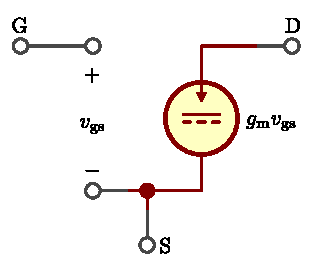
\includegraphics{../assets/small_signal.pdf}
        \caption{Small-signal equivalent circuit of a MOSFET.}
        \label{fig:mosfet_small_signal_model}
    \end{figure}
    \begin{align*}
        i_{\mathrm{g}}(v_{\mathrm{gs}}, v_{\mathrm{ds}}) &= 0 \\
        i_{\mathrm{d}}(v_{\mathrm{gs}}, v_{\mathrm{ds}}) &= g_{\mathrm{m}}v_{\mathrm{gs}}
    \end{align*}
\end{frame}
\note[itemize]{
    \item Open connection between gate and source, gate current zero
    \item Linear voltage controlled current source between drain and source
    \item Enough theory to analyze circuits
}